% Title:       Uniflow (unified workflow)
% Author:      Leo Arnold
% URL:         https://github.com/leoarnold/uniflow-dante2013
% License:     CC BY 4.0 - http://creativecommons.org/licenses/by/4.0/

\documentclass[]{beamer}

\usepackage[ngerman]{babel}
\usepackage[utf8]{inputenc}
\usepackage[T1]{fontenc}

\usepackage{csquotes, listings}
  \lstdefinestyle{arn:lst}{basicstyle=\scriptsize, breaklines=true, commentstyle=\itshape\color{gray}}
  \lstdefinestyle{arn:lst:tex}{backgroundcolor=\color{gray!20}, frame=single, language={[LaTeX]TeX}, style=arn:lst}
  \lstdefinestyle{arn:lst:bash}{language=Bash, basicstyle=\ttfamily, showstringspaces=false, style=arn:lst}

\usetheme{Boadilla}
\setbeamertemplate{navigation symbols}{}

\AtBeginSection{
\begin{frame}
  \frametitle{Wo sind wir gerade?}
  \tableofcontents[currentsection, hideothersubsections]
\end{frame}}

\begin{document}
\title{UniFlow (\underline{uni}fied work\underline{flow})}
\subtitle{Wie man mit nur einem \LaTeX{}-Durchlauf\\ mehrere Dokumente erzeugen kann}
\author{Leo Arnold}
\institute{tex@arney.de}
\date{Dante Frühjahr 2013}

\begin{frame}
  \titlepage
\end{frame}

\begin{frame}
  \frametitle{Das ist der Plan}
  \tableofcontents[hideallsubsections]
\end{frame}

\section{Die Wurzel allen Übels}

\begin{frame}
\frametitle{Wozu mehrere Dokumente aus derselben Quelle?}

\vfill

\begin{center}
\begin{tabular}{cp{1em}c}
\texttt{Blatt01-Angabe.pdf} & \strut & \texttt{Blatt01-MuLoe.pdf}\\
\fbox{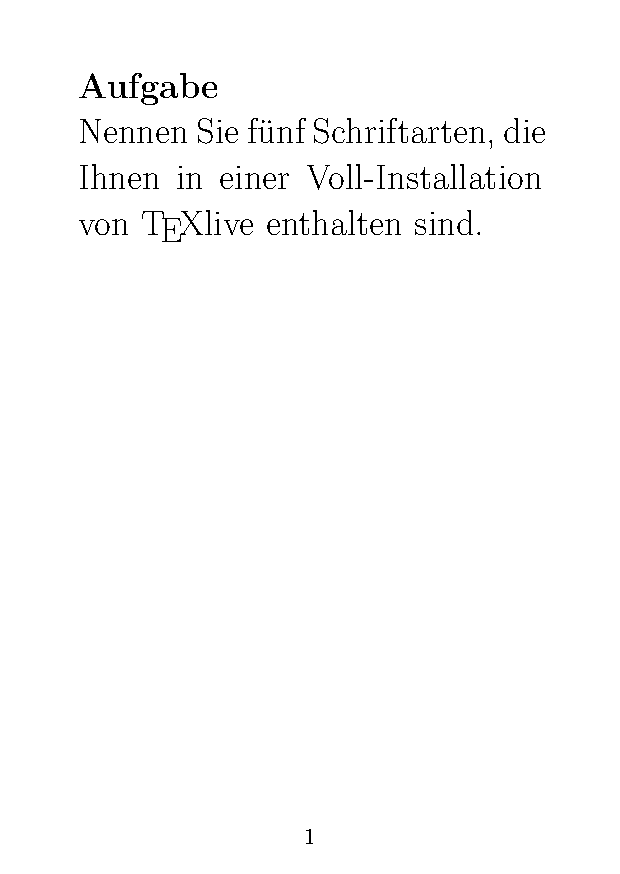
\includegraphics[height=.7\paperheight]{pic/Blatt01-Angabe}}
&& \fbox{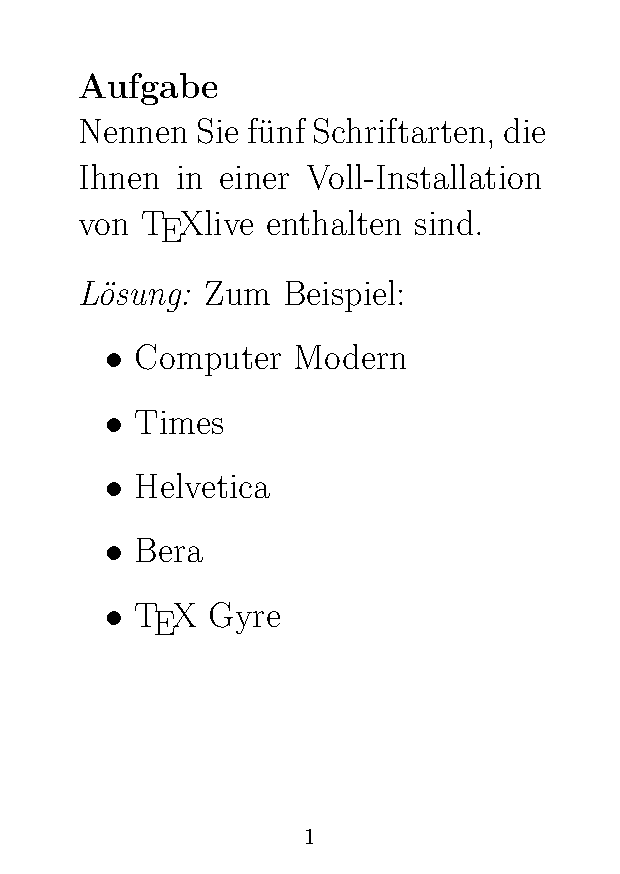
\includegraphics[height=.7\paperheight]{pic/Blatt01-MuLoe}}
\end{tabular}
\end{center}

\vfill

\end{frame}

\begin{frame}
\frametitle{... und dieses Problem lösen wir nebenbei auch}

\begin{center}
  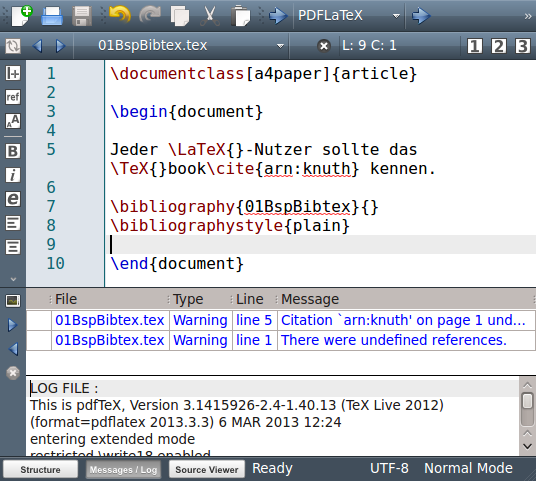
\includegraphics[height=.8\paperheight]{pic/FindeDenFehler}
\end{center}

\end{frame}

\begin{frame}
\frametitle{Konzeptioneller Fehler}

\begin{center}
  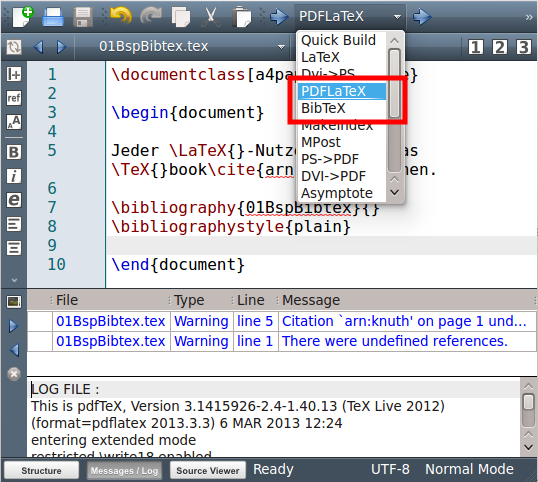
\includegraphics[height=.8\paperheight]{pic/FehlerImKonzept}
\end{center}

\end{frame}

\begin{frame}
\frametitle{UniFlow is not Unix...}

Ein \LaTeX{}-Aufruf erstellt nur ein Ausgabedokument. Gängige Behelfe:
\begin{itemize}[<+->]
\item Shell Skript
\item MakeFile
\item Pseudo-executables
\item Irgendwas mit LUA.
\end{itemize}
\pause\medskip ... aber andererseits
\begin{itemize}[<+->]
\item benötigt eine extra Skript-Datei
\item benötigt Programme jenseits von \TeX{}live
\item ist meist nicht plattform-unabhängig
\item benötigt Programmierkenntnisse jenseits der \TeX{}-Syntax
\end{itemize}
\pause\medskip Geht das nicht auch allein mit pdf\LaTeX{}?
\end{frame}

\section{Der Weg zum UniFlow-Prinzip}

\begin{frame}
\frametitle{Anforderungen}

\begin{itemize}[<+->]
\item Nur \textbf{ein} Quelldokument
\begin{itemize}[<+->]
\item natürliche Arbeitsweise: Lösung unmittelbar unter die Aufgabe tippen
\item keine Duplikate: Wiederverwenden statt Rüberkopieren
\item Kongruenz aller Änderungen: \enquote{Alle ersetzen} ändert Angabe und Lösung
\end{itemize}
\item Einfache Wiederverwendung einzelner Aufgaben
\begin{itemize}[<+->]
\item Aufteilung mit \texttt{\textbackslash{}include} soll weiterhin möglich sein
\item Rechenaufgaben: Binde Mathe-Software ein und automatisiere Berechnungen
\end{itemize}
\end{itemize}

\end{frame}

\begin{frame}
\frametitle{Man nehme...}

\vfill

\begin{enumerate}[<+->]
\item Quellcode gezielt einbinden
\item Wiederentdeckung der Kommandozeile
\item Namen des Ausgabedokuments ändern
\item Ausbrechen auf die Shell
\item Pseudo Shell-Scripts in \LaTeX\
\end{enumerate}

\vfill
\end{frame}

\begin{frame}[fragile]
\frametitle{Quellcode gezielt einbinden}
\framesubtitle{Ein wertvoller Tipp von Rolf Niepraschk}

Benutze das Paket \texttt{comment.sty} von Victor Eijkhout.

\pause

\begin{itemize}
\item \verb+\includecomment{foobar}+\\
Definiert die Umgebung \texttt{foobar}, deren Inhalt eingebunden wird
\item \verb+\excludecomment{foobar}+\\
Definiert die Umgebung \texttt{foobar}, deren Inhalt auskommentiert wird
\end{itemize}

\pause\hfill
\begin{minipage}{0.45\linewidth}
\begin{lstlisting}[style=arn:lst:tex]
\includecomment{wahrheit}
\excludecomment{nonsens}

Knuth begann mit
\begin{wahrheit}
der Entwicklung von \TeX{}
\end{wahrheit}
\begin{nonsens}
unter Verwendung von WinWord
\end{nonsens}
im Jahr 1977.
\end{lstlisting}
\end{minipage}
\hfill\strut

\pause\textbf{Ausgabe:} \: Knuth begann mit der Entwicklung von \TeX{} im Jahr 1977.


\end{frame}

\begin{frame}[fragile]
\frametitle{Anwendung bei Übungsblättern}

Als Schalter definieren wir später das Makro \verb+\condition+

\begin{center}
\begin{minipage}{0.45\linewidth}
\begin{lstlisting}[style=arn:lst:tex, title={\texttt{Blatt01.tex}}]
\RequirePackage{comment}

\includecomment{problem}
\ifcase\condition
  % \condition = 0, Angabe
  \includecomment{aufgabe}
  \excludecomment{loesung}
\or % \condition = 1, MuLoe
  \includecomment{aufgabe}
  \includecomment{loesung}
\fi

% LaTeX-Dokument hier
\end{lstlisting}
\end{minipage}
\end{center}

Wir benötigen \verb+\RequirePackage+, da dieser Code-Block noch vor \verb+\documentclass+ stehen soll.
\end{frame}

\begin{frame}[fragile]
\frametitle{Wiederentdeckung der Kommandozeile}
\framesubtitle{Ein wertvoller Tipp von R.~J. Drofnats}

Wir könnten nun \verb+\condition+ in einem Wrapper-Dokument setzen:

\begin{center}
\begin{minipage}{0.45\linewidth}
\begin{lstlisting}[style=arn:lst:tex]
\gdef\condition{0}
\input Blatt01
\end{lstlisting}
\end{minipage}
\end{center}

aber das wäre eine weitere Datei.\pause{} Es geht aber auch ohne:

\begin{center}
\begin{minipage}{0.8\linewidth}
\begin{lstlisting}[style=arn:lst:bash]
pdflatex "\gdef\condition{0} \input Blatt01"
\end{lstlisting}
\end{minipage}
\end{center}

\pause Dabei können wir den Namen des Ausgabedokuments gleich anpassen:

\begin{center}
\begin{minipage}{0.8\linewidth}
\begin{lstlisting}[style=arn:lst:bash]
pdflatex --jobname=Blatt01-Angabe "\gdef\condition{0} \input Blatt01"
\end{lstlisting}
\end{minipage}
\end{center}

\end{frame}

\begin{frame}[fragile]
\frametitle{Ausbrechen auf die Shell}

pdf\LaTeX\ kann Befehle direkt auf die Kommandozeile schreiben:

\begin{center}
\begin{minipage}{0.45\linewidth}
\begin{lstlisting}[style=arn:lst:tex]
\write18{ping www.dante.de}
\end{lstlisting}
\end{minipage}
\end{center}

\pause Das werden wir gleich auf das Gelernte anwenden, doch zuvor:

\pause\bigskip

\textbf{Warnung:} Zugriff auf die Shell ist eine \alert{Sicherheitslücke}.
Daher ist \verb+\write18+ grundsätzlich gesperrt. Nur bei Verwendung von
\begin{center}
\begin{minipage}{0.45\linewidth}
\begin{lstlisting}[style=arn:lst:bash]
pdflatex --shell-escape
\end{lstlisting}
\end{minipage}
\end{center}
wird der Befehl für diesen Durchlauf aktiviert.
\end{frame}


\begin{frame}[fragile]
\frametitle{Pseudo Shell-Scripts in \LaTeX{}}
\framesubtitle{Ein wertvoller Tipp von Ulrike Fischer (TeX.SX \#5265)}

\begin{center}
\begin{minipage}{0.8\linewidth}
\begin{lstlisting}[title={Blatt01.tex}, style=arn:lst:tex]
\ifx\condition\undefined
  \immediate\write18{
    pdflatex --jobname=\jobname-Angabe
    "\gdef\string\condition{0}
     \string\input\space\jobname"
  }
  % weitere Faelle hier
  \expandafter\stop
\fi

% Fallunterscheidung hier

% LaTeX-Dokument hier
\end{lstlisting}
\end{minipage}
\end{center}

\pause
\begin{itemize}[<+->]
\item \verb+\immediate+: sofort ausführen, dann erst weiter parsen
\item \verb+\expandafter+: erst \verb+\fi+ noch lesen, dann \verb+\stop+
\item \verb+\stop+: Sofortiger Abbruch
\end{itemize}

\end{frame}

\begin{frame}[fragile]
\frametitle{Zusammenfassung: UniFlow-Prinzip}

\begin{enumerate}[<+->]
\item Wir starten mit
\begin{lstlisting}[style=arn:lst:bash]
pdflatex --shell-escape Blatt01.tex
\end{lstlisting}
\item Dieser Durchlauf ruft
\begin{lstlisting}[style=arn:lst:bash]
pdflatex --jobname=Blatt01-Angabe "\gdef\condition{0} \input Blatt01.tex"
pdflatex --jobname=Blatt01-MuLoe "\gdef\condition{1} \input Blatt01.tex"
\end{lstlisting}
auf und stoppt danach sofort.
\item Die Aufrufe aus Schritt 2 erzeugen je ein Ausgabedokument mit den gewünschten Optionen aus ein- und derselben Quelldatei.
\end{enumerate}
\end{frame}

\section{Showcase und Live-Demos}

\begin{frame}[fragile]
\frametitle{Lösung des zweiten Eingangsbeispiels}

\begin{center}
\begin{lstlisting}[style=arn:lst:tex]
\ifx\condition\undefined
  \immediate\write18{
   pdflatex "\gdef\string\condition{0} \string\input\space\jobname"
  }
  \immediate\write18{
   bibtex "\jobname"
  }
  \immediate\write18{
   pdflatex "\gdef\string\condition{0} \string\input\space\jobname"
  }
    \immediate\write18{
   pdflatex "\gdef\string\condition{0} \string\input\space\jobname"
  }
  \expandafter\stop
\fi

% LaTeX-Dokument hier
\end{lstlisting}
\end{center}

Hier wird \verb+\condtion+ nur definiert, um den \verb+\ifx+-Block zu überspringen. Da wir nur eine Version erstellen, entfällt die Fallunterscheidung.

\end{frame}

\begin{frame}[fragile]
\frametitle{Algebra mit Sage}

\begin{minipage}{.45\linewidth}
\fbox{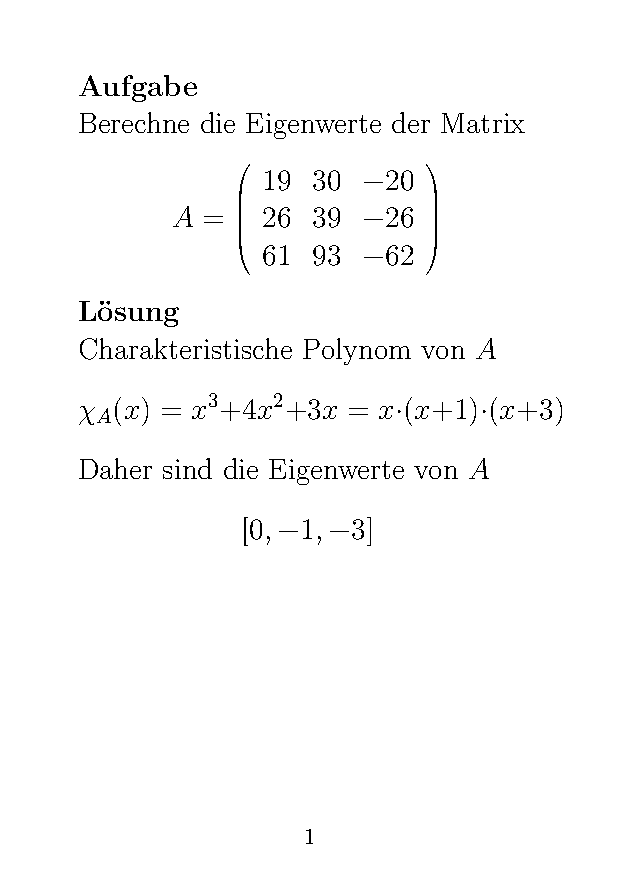
\includegraphics[height=.75\paperheight]{pic/BspAlgebra}}
\end{minipage}
\hfill
\begin{minipage}{.45\linewidth}
\textbf{Workflow}
\begin{lstlisting}[style=arn:lst:bash]
pdflatex BspAlgebra.tex
sage BspAlgebra.sagetex.sage
pdflatex BspAlgebra.tex
\end{lstlisting}

\bigskip

\textbf{Inspiration}\\
Günter Rau, \enquote{Sage\TeX{}},\\ \href{http://archiv.dante.de/DTK/PDF/komoedie_2011_1.pdf}{DTK 2011-1}, p. 17ff

\end{minipage}

\end{frame}

\begin{frame}[fragile]
\frametitle{Statistik mit GNU R}

\begin{minipage}{.45\linewidth}
\fbox{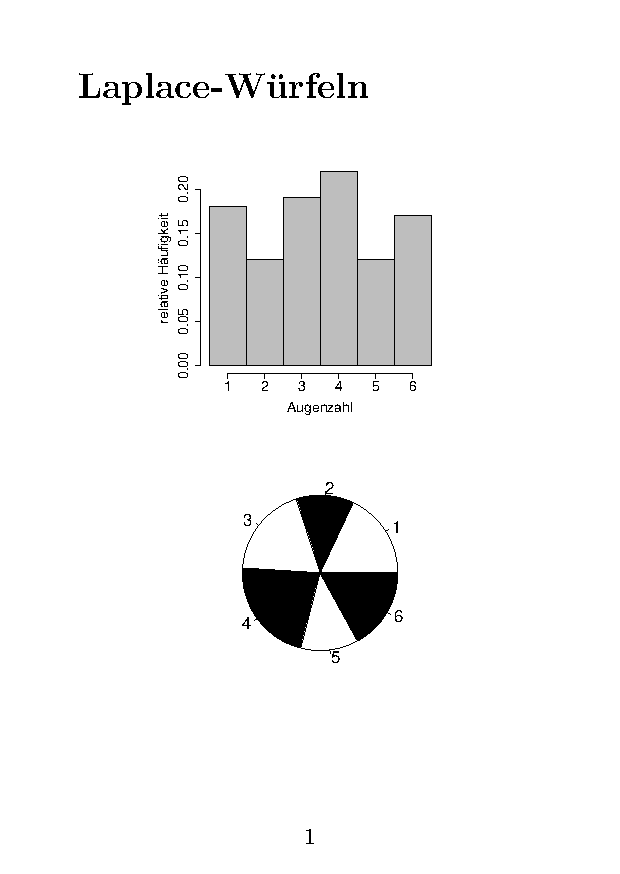
\includegraphics[height=.75\paperheight]{pic/BspStatistik}}
\end{minipage}
\hfill
\begin{minipage}{.45\linewidth}
\textbf{Workflow}
\begin{lstlisting}[style=arn:lst:bash]
R CMD Sweave BspStatistik.Rnw
pdflatex BspStatistik.tex
\end{lstlisting}

\bigskip

\textbf{Inspiration}\\
Uwe Ziegenhagen, \enquote{Datenanalyse mit Sweave, \LaTeX\ und R},\\ \href{http://www.dante.de/DTK/Ausgaben/dtk104.pdf}{DTK 2010-4}, p. 35ff
\end{minipage}

\end{frame}

\end{document}